\begin{figure}[ht]
  \centering
  \resizebox{.8\linewidth}{!}{
    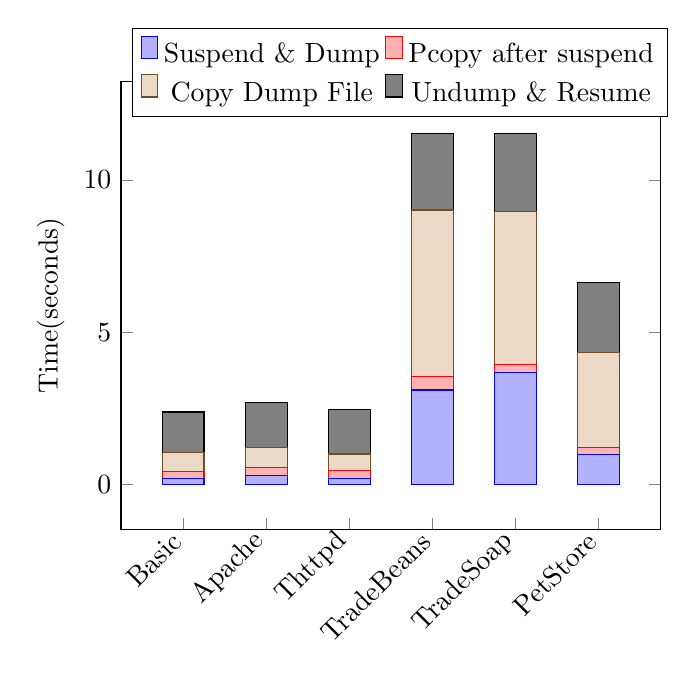
\begin{tikzpicture}
      \begin{axis}[
        ybar stacked,
        bar width=15pt,
        %	nodes near coords,
        enlargelimits=0.15,
        legend style={at={(0.02,1.12)},anchor=north west,legend columns=2},
        ylabel={Time(seconds)},
        symbolic x coords={Basic, Apache, Thttpd, TradeBeans, TradeSoap, 
          PetStore},
        xtick=data,
        x tick label style={rotate=45,anchor=east},
        ]
        \addplot+[ybar] plot coordinates {(Basic,0.21) (Apache,0.30) (Thttpd,0.21) (TradeBeans,3.10) (TradeSoap,3.68) (PetStore,0.97) };
        \addplot+[ybar] plot coordinates {(Basic,0.22) (Apache,0.27) (Thttpd,0.26) (TradeBeans,0.44) (TradeSoap,0.25) (PetStore,0.24) };
        \addplot+[ybar] plot coordinates {(Basic,0.62) (Apache,0.64) (Thttpd,0.53) (TradeBeans,5.47) (TradeSoap,5.03) (PetStore,3.11) };
        \addplot+[ybar] plot coordinates {(Basic,1.33) (Apache,1.47) (Thttpd,1.46) (TradeBeans,2.51) (TradeSoap,2.57) (PetStore,2.32) };
        \addlegendentry{\strut Suspend \& Dump}
        \addlegendentry{\strut Pcopy after suspend}
        \addlegendentry{\strut Copy Dump File}
        \addlegendentry{\strut Undump \& Resume}
      \end{axis}
    \end{tikzpicture}
   }
  %\captionsetup{justification=centering}
  \caption{Suspend time for live cloning, when running a representative benchmark}
  \label{fig:stats}
\end{figure}


\subsubsection{Real world applications and workloads:}
To begin to study the overhead of live cloning, we performed an evaluation using five well-known applications.
Figure~\ref{fig:stats} presents the suspended times for five well-known applications when cloning a replica with \parikshan. 
We ran the httperf~\cite{httperf} benchmark on Apache and \emph{thttpd} to compute max throughput of the web-servers, by sending a large number of concurrent requests.
Tradebeans and Tradesoap are both part of the dacapo~\cite{dacapo} benchmark ``DayTrader'' application.
These are realistic workloads, which run on a multi-tier trading application provided by IBM. 
PetStore~\cite{petstore} is also a well known J2EE reference application. 
We deployed PetStore in a 3-tier system with JBoss, MySQL and Apache servers, and cloned the app-server.
The input workload was a random set of transactions which were repeated for the duration of the cloning process.

As shown in Figure~\ref{fig:stats}, for Apache and Thttpd the container suspend time ranged between 2-3 seconds.
However, in more memory intensive application servers such as PetStore and DayTrader, the total suspend time was higher (6-12 seconds).
Nevertheless, we did not experience any timeouts or errors for the requests in the workload\footnote{In case of packet drops, requests are resent both at the TCP layer, and the application layer. This slows down the requests for the user, but does not drop them}.
However, this did slowdown requests in the workload. 
This shows that short suspend times are largely not visible or have minimal performance impact to the user, as they are within the time out range of most applications.
Further, a clean network migration process ensures that connections are not dropped, and are executed successfully.
We felt that these relatively fast temporary app suspensions were a reasonable price to pay to launch an otherwise overhead-free debug replica.
To further characterize the suspend time imposed by the live cloning phase of \parikshan, we created a synthetic micro-benchmark to push \parikshan towards its limit.